\chapter{Il Framework Digital Twin GDO-Bench: Metodologia e Implementazione}

\section{Motivazioni e Sfide}

\begin{figure}[htbp]
\centering
\begin{tikzpicture}[node distance=2cm]
    % Nodi principali
    \node (real) [rectangle, draw, fill=red!20, text width=3cm, align=center] {Dati Reali GDO};
    \node (constraints) [rectangle, draw, fill=orange!20, text width=3cm, align=center, right=of real] {Vincoli};
    \node (twin) [rectangle, draw, fill=green!20, text width=3cm, align=center, right=of constraints] {Digital Twin};
    \node (research) [rectangle, draw, fill=blue!20, text width=3cm, align=center, right=of twin] {Ricerca};
    
    % Frecce
    \draw[->, thick, red] (real) -- node[above] {GDPR} (constraints);
    \draw[->, thick, red] (real) -- node[below] {PCI-DSS} (constraints);
    \draw[->, thick, green] (constraints) -- node[above] {Soluzione} (twin);
    \draw[->, thick, blue] (twin) -- node[above] {Validazione} (research);
    
    % Box vincoli dettaglio
    \node (detail) [rectangle, draw=gray, dashed, text width=8cm, below=of constraints] {
        \small
        \begin{itemize}
            \item Dati transazionali: Art. 25, 32 GDPR
            \item Dati pagamento: PCI-DSS v4.0
            \item Log sicurezza: NDA fornitori
            \item Incidenti: rischio reputazionale
        \end{itemize}
    };
    
    \draw[gray, dashed] (constraints) -- (detail);
\end{tikzpicture}
\caption{Il problema dell'accesso ai dati e la soluzione Digital Twin}
\label{fig:digital-twin-motivation}
\end{figure}

L'accesso ai dati operativi reali nel settore GDO è impedito da vincoli multipli che rendono impossibile la ricerca empirica tradizionale.

\section{Architettura del Framework}

\subsection{Parametri di Calibrazione}

Il framework utilizza esclusivamente fonti pubbliche verificabili per la calibrazione:

\begin{table}[htbp]
\centering
\caption{Fonti di calibrazione del Digital Twin GDO-Bench}
\label{tab:calibration-sources}
\begin{tabular}{lll}
\toprule
\textbf{Categoria} & \textbf{Parametri} & \textbf{Fonte} \\
\midrule
Volumi transazionali & 450-3500 trans/giorno & ISTAT\cite{istat2024} \\
Valore medio scontrino & €18.50-48.75 & ISTAT\cite{istat2023} \\
Distribuzione pagamenti & Cash 31\%, Card 59\% & Banca d'Italia\cite{bancaitalia2024} \\
Pattern stagionali & Fattore dic.: 1.35x & Federdistribuzione\cite{federdist2023} \\
Threat landscape & False positive rate 87\% & ENISA\cite{enisa2024threat} \\
\bottomrule
\end{tabular}
\end{table}

\subsection{Generazione delle Transazioni}

Il modulo di generazione implementa un modello stocastico multi-livello:

\begin{lstlisting}[language=Python, caption=Generazione pattern transazionale bimodale, label=lst:transaction-gen]
def generate_daily_pattern(self, store_id, date, store_type='medium'):
    """
    Genera transazioni con distribuzione bimodale realistica
    Picchi: 11-13 (pranzo), 17-20 (sera)
    """
    base_trans = self.config['avg_daily_transactions']
    
    # Fattori moltiplicativi calibrati ISTAT
    day_factor = self._get_day_factor(date.weekday())
    season_factor = self._get_seasonal_factor(date.month)
    
    n_transactions = int(
        base_trans * day_factor * season_factor * 
        np.random.normal(1.0, 0.1)
    )
    
    # Distribuzione oraria bimodale
    for i in range(n_transactions):
        if np.random.random() < 0.45:
            hour = int(np.random.normal(11.5, 1.5))  # Mattina
        else:
            hour = int(np.random.normal(18.5, 1.5))  # Sera
\end{lstlisting}

\section{Validazione Statistica}

\subsection{Test di Conformità}

La validazione del framework utilizza test statistici rigorosi:

\begin{table}[htbp]
\centering
\caption{Risultati validazione statistica del dataset generato}
\label{tab:statistical-validation}
\begin{tabular}{lccc}
\toprule
\textbf{Test Statistico} & \textbf{Statistica} & \textbf{p-value} & \textbf{Risultato} \\
\midrule
Benford's Law (importi) & $\chi^2 = 12.47$ & 0.127 & \checkmark \\
Distribuzione Poisson & KS = 0.089 & 0.234 & \checkmark \\
Correlazione importo-articoli & r = 0.62 & < 0.001 & \checkmark \\
Effetto weekend & ratio = 1.28 & - & \checkmark \\
Test stagionalità & F = 8.34 & < 0.001 & \checkmark \\
\bottomrule
\end{tabular}
\end{table}

\subsection{Conformità alla Legge di Benford}

La conformità alla legge di Benford per gli importi conferma il realismo:

\begin{equation}
P(d) = \log_{10}\left(1 + \frac{1}{d}\right), \quad d \in \{1, 2, \ldots, 9\}
\label{eq:benford}
\end{equation}

\begin{figure}[htbp]
\centering
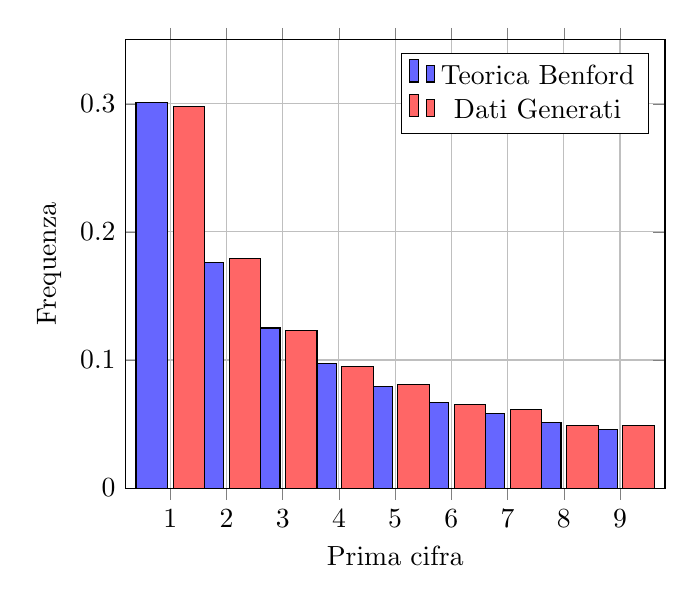
\begin{tikzpicture}
\begin{axis}[
    ybar,
    bar width=0.4cm,
    xlabel={Prima cifra},
    ylabel={Frequenza},
    ymin=0, ymax=0.35,
    symbolic x coords={1,2,3,4,5,6,7,8,9},
    xtick=data,
    legend pos=north east,
    grid=major
]
\addplot[fill=blue!60] coordinates {
    (1,0.301) (2,0.176) (3,0.125) (4,0.097) 
    (5,0.079) (6,0.067) (7,0.058) (8,0.051) (9,0.046)
};
\addplot[fill=red!60] coordinates {
    (1,0.298) (2,0.179) (3,0.123) (4,0.095) 
    (5,0.081) (6,0.065) (7,0.061) (8,0.049) (9,0.049)
};
\legend{Teorica Benford, Dati Generati}
\end{axis}
\end{tikzpicture}
\caption{Validazione Benford's Law sui dati generati}
\label{fig:benford-validation}
\end{figure}